\documentclass[12pt,a4paper,oneside]{report}             % Single-side
%\documentclass[11pt,a4paper,twoside,openright]{report}  % Duplex

\PassOptionsToPackage{chapternumber=Huordinal}{magyar.ldf}
\usepackage[utf8]{inputenc}
\usepackage[T1]{fontenc}
\def\magyarOptions{defaults=hu-min,suggestions=no}
\usepackage{amsmath}
\usepackage{amssymb}
\usepackage{enumerate}
\usepackage{enumitem}
\usepackage[thmmarks]{ntheorem}
\usepackage{graphics}
\usepackage{epsfig}
\usepackage{listings}
\usepackage{color}
%\usepackage{fancyhdr}
\usepackage{lastpage}
\usepackage{anysize}
\usepackage{footnote}
\usepackage[magyar]{babel}
\usepackage{csquotes}
\usepackage{sectsty}
\usepackage{setspace}  % Ettől a táblázatok, abrak, lábjegyzetek maradnak 1-es sorközzel!
\usepackage[hang]{caption}
\usepackage{xcolor}
\usepackage{blindtext}
\usepackage{scrextend}
\usepackage{tikz}
\usepackage{aeguill}
\usepackage{microtype}
\usepackage{interval}
\usepackage{graphicx}
\usepackage[unicode]{hyperref}
\addtokomafont{labelinglabel}{\sffamily}
\usepackage[
backend=biber,
style=alphabetic,
sorting=nyt
]{biblatex}
\addbibresource{mybib.bib}

%--------------------------------------------------------------------------------------
% Main variables
%--------------------------------------------------------------------------------------
\newcommand{\vikszerzo}{Zih Botond}
\newcommand{\vikkonzulens}{Dr.~Antal Péter}
\newcommand{\vikcim}{Bayes-hálók tanulása paraméterek diszkretizálásának integrálásával}
\newcommand{\viktanszek}{Méréstechnika és Információs Rendszerek Tanszék}
\newcommand{\vikdoktipus}{Diplomamunka}
\newcommand{\argmin}{\mathop{\mathrm{arg\,min}}}
\newcommand\descitem[1]{\item{\bfseries #1}}

%--------------------------------------------------------------------------------------
% Page layout setup
%--------------------------------------------------------------------------------------
% we need to redefine the page style plain
% another possibility is to use the body of this command without \fancypagestyle
% and use \pagestyle{fancy} but in that case the special pages
% (like the ToC, the References, and the Chapter pages)remain in plane style

\pagestyle{plain}
%\setlength{\parindent}{0pt} % áttekinthetőbb, angol nyelvű dokumentumokban jellemző
%\setlength{\parskip}{8pt plus 3pt minus 3pt} % áttekinthetőbb, angol nyelvű dokumentumokban jellemző
\setlength{\parindent}{12pt} % magyar nyelvű dokumentumokban jellemző
\setlength{\parskip}{0pt}    % magyar nyelvű dokumentumokban jellemző

\marginsize{35mm}{25mm}{15mm}{15mm} % any size package
\setcounter{secnumdepth}{0}
\sectionfont{\large\upshape\bfseries}
\setcounter{secnumdepth}{2}
\singlespacing
\frenchspacing

%--------------------------------------------------------------------------------------
%	Setup hyperref package
%--------------------------------------------------------------------------------------
\hypersetup{
    %bookmarks=true,            % show bookmarks bar?
    %unicode=false,             % non-Latin characters in Acrobat’s bookmarks
    pdftitle={\vikcim},        % title
    pdfauthor={\vikszerzo},    % author
    pdfsubject={\vikdoktipus}, % subject of the document
    pdfcreator={\vikszerzo},   % creator of the document
    pdfproducer={Producer},    % producer of the document
    pdfkeywords={keywords},    % list of keywords
    pdfnewwindow=true,         % links in new window
    colorlinks=true,           % false: boxed links; true: colored links
    linkcolor=black,           % color of internal links
    citecolor=black,           % color of links to bibliography
    filecolor=black,           % color of file links
    urlcolor=black             % color of external links
}

%--------------------------------------------------------------------------------------
% Set up listings
%--------------------------------------------------------------------------------------
\lstset{
	basicstyle=\scriptsize\ttfamily, % print whole listing small
	keywordstyle=\color{black}\bfseries\underbar, % underlined bold black keywords
	identifierstyle=, 					% nothing happens
	commentstyle=\color{white}, % white comments
	stringstyle=\scriptsize\sffamily, 			% typewriter type for strings
	showstringspaces=false,     % no special string spaces
	aboveskip=3pt,
	belowskip=3pt,
	columns=fixed,
	backgroundcolor=\color{lightgray},
}
\def\lstlistingname{lista}

%--------------------------------------------------------------------------------------
%	Some new commands and declarations
%--------------------------------------------------------------------------------------
\newcommand{\code}[1]{{\upshape\ttfamily\scriptsize\indent #1}}

% define references
\newcommand{\figref}[1]{\ref{fig:#1}.}
\renewcommand{\eqref}[1]{(\ref{eq:#1})}
\newcommand{\listref}[1]{\ref{listing:#1}.}
\newcommand{\sectref}[1]{\ref{sect:#1}}
\newcommand{\tabref}[1]{\ref{tab:#1}.}

\DeclareMathOperator*{\argmax}{arg\,max}
%\DeclareMathOperator*[1]{\floor}{arg\,max}
\DeclareMathOperator{\sign}{sgn}
\DeclareMathOperator{\rot}{rot}
\definecolor{lightgray}{rgb}{0.95,0.95,0.95}

\author{\vikszerzo}
\title{\viktitle}
%--------------------------------------------------------------------------------------
%	Setup captions
%--------------------------------------------------------------------------------------
\captionsetup[figure]{
%labelsep=none,
%font={footnotesize,it},
%justification=justified,
width=.75\textwidth,
aboveskip=10pt}

\renewcommand{\captionlabelfont}{\small\bf}
\renewcommand{\captionfont}{\footnotesize\it}

%--------------------------------------------------------------------------------------
% Table of contents and the main text
%--------------------------------------------------------------------------------------
\begin{document}
\singlespacing

\pagenumbering{arabic}
\onehalfspacing
%--------------------------------------------------------------------------------------
%	The title page
%--------------------------------------------------------------------------------------
\begin{titlepage}
\begin{center}

\includegraphics[width=60mm,keepaspectratio]{figures/BMElogo.png}\\
\vspace{0.3cm}
\textbf{Budapesti Műszaki és Gazdaságtudományi Egyetem}\\
\textmd{Villamosmérnöki és Informatikai Kar}\\
\textmd{\viktanszek}\\[5cm]

\vspace{0.4cm}
{\huge \bfseries \vikcim}\\[0.8cm]
\vspace{0.5cm}
\textsc{\Large \vikdoktipus}\\[4cm]

\begin{tabular}{cc}
 \makebox[7cm]{\emph{Készítette}} & \makebox[7cm]{\emph{Konzulens}} \\
 \makebox[7cm]{\vikszerzo} & \makebox[7cm]{\vikkonzulens}
\end{tabular}

\vfill
{\large \today}
\end{center}
\end{titlepage}



\tableofcontents\vfill
%----------------------------------------------------------------------------
\chapter*{Bevezetés}\addcontentsline{toc}{chapter}{Bevezetés}
%----------------------------------------------------------------------------
Kauzalitás modellezésére gyakori a Bayes-hálók használata. Ezen modellek a diszkrét változók közötti kapcsolatot írják le. Ezért a tanításukat is diszkrét adatokon kell végezni. A mérhető, nyers adatok azonban gyakran tartalmaznak folytonos változókat. Ezeknek a diszkretizálására újabb eljárások kifejlesztése továbbra is folyamatban van. Jelen Diplomamunka az egyik új diszkretizációs eljárás köré épül és egy automatizált Bayes-háló tanító könyvtárat mutat be, mely ezt az eljárást használja. Az új eljárást Chen et al. publikálta \cite{chen2017learning}.

Az orvosi laboratóriumi diagnosztika területe az egyik felhasználója a kauzalitásos modelleknek. Ennek oka, hogy a betegség és tünetek összefüggéseire építhetők Bayes-hálók. A tünetek pedig a vérképben is megjelenhetnek. Így a vérben és más testnedvekben található részecskék tulajdonságait, koncentrációját mérve felderíthetők betegségek, ha van ezekhez készült modell. A mért változók a laboratóriumi paraméterek, és mivel ezek mért eredmények, diszkretizálandók. Ezért az új eljárást ilyen típusú adatokon is tesztelendő.

A Diplomamunkának három kitűzött célja van. Az első a jelenlegi diszkretizációs módszerek bemutatása. Ehhez a felhasznált algoritmusok, kifejezések magyarázatára is szükség van. A második a referenciamódszer implementálásának bemutatása. A harmadik az elkészült rendszerrel szintetikus és valós adatsorok kiértékelése, az eredmények bemutatása és értelmezése. A valós adatok tartalmazzanak laboratóriumi paramétereket, és az eljárás használhatóságát vizsgálja ilyen esetekben.

A Bevezetés fejezet tartalmazza a Diplomamunka célját, szerkezetét és a fő fejezetek tartalmát. Ez segít a dokumentum átlátásában.

A Fogalommagyarázat című fejezetben szerepelnek a statisztikai alapfogalmak. Később csak hivatkozás történik ezekre, ismeretük szükséges az algoritmus megértéséhez.

A Valószínűségelmélet fejezet összefoglalja a bayesiánus statisztika azon részeit, melyeket a Diplomamunka később használ. Emellett példákat ad a könnyebb befogadáshoz. Itt szerepel az algoritmus megértéséhez szükséges Bayes-i következtetés ismertetése, valamint a Bayes-hálókról adott áttekintés.

A Jelenlegi módszerek fejezetben a diszkretizációs algoritmusokról szerepel egy áttekintés. Bemutatja a különbséget az egyváltozós és a többváltozós diszkretizáció között. A Bayes-hálók tanításához a struktúrájának a meghatározása is szükséges, erre a célra készült algoritmusok is bemutatásra kerülnek.

Az Algoritmikus többváltozós diszkretizáció fejezetben a Diplomamunka referenciájaként szolgáló módszer leírása szerepel. Emellett a használt algoritmusokat kifejti, a lépések feladatát értelmezi. Az itt szereplő módszer az elkészült implementáció központi eleme.

A Bayes-döntés alapján diszkretizáló csomag fejezet dokumentálja az elkészült csomagot. Részletesen kifejtett követelmények szerepelnek, amik az implementációs célokat tűzik ki. Bemutatja a rendszer felépítését és működését.

A Kiértékelés szintetikus adatokon fejezet mutatja be az elkészült implementációval végzett kísérleteket, az ismertetett algoritmusok összehasonlítását. Végül értékeli az összehasonlítások eredményét.

A Kiértékelés valós adatokon fejezet laboratóriumi mérések adatain teszteli a rendszert. Bemutatja a diszkretizációs módszer működését laborparamétereket tartalmazó adatsoron, és értékeli a használhatóságát.

A lebegőpontos számok tizedesvessző helyett tizedesponttal szerepelnek.
%----------------------------------------------------------------------------
\chapter{Fogalommagyarázat}
%----------------------------------------------------------------------------

Az alábbi fejezet a Diplomamunkában használt fogalmak jelentését, a megértéshez szükséges alapismereteket foglalja össze.

\section{Előfeldolgozás}
Egy statisztikai feldolgozásra kapott adatsoron nem alkalmazhatóak azonnal statisztikai módszerek. Az adatsorban különböző hibák előfordulhatnak. Ilyenek lehetnek:
\begin{itemize}
    \item Hiányok
    \item Nem megfelelő típusú értékek
    \item Inkonzisztens adatok
\end{itemize}
Ezért a statisztikai vizsgálat előtt szükség van egy \emph{előfeldolgozás}i lépésre, amely során előáll az adatok megfelelő formája.

\section{Statisztikai változó, adatpont}
A statisztikai számításnál rendezett adatsorokat használunk. A rendezettség a sorokra és oszlopokra bontott adatokban jelenik meg. Ezért az adathalmaz felírható táblázatos formában. A táblázat oszlopai a statisztikai változók, vagy röviden \emph{változó}k. Ezeket a tulajdonságokat értékeljük ki a vizsgált entitásoknál. Az oszlopban szereplő értékek egyforma típusúak (szám, szöveg), értelmezésük azonos. Amennyiben egy fizikai mennyiséget ábrázol, akkor a mértékegysége minden értéknek azonos, vagy egyértelműen jelölt. Ha a mértékegységek különböznek, az előfeldolgozás során célszerű ugyanolyan mértékegységre váltani őket.

Az adatsor soraiban egy egyedhez tartozó értékek szerepelnek. Ezek jellemzik az adott egyedet az adatsor változói szerint. Az egyed tágabban is értelmezhető, nem szükséges hozzá a valódi világnak egy objektuma, de az egy sorban szereplő adatoknak kapcsolódniuk kell egymáshoz. Egy sort \emph{adatpont}nak is neveznek, mert a változók által kifeszített térben pontosan egy pontot jelöl ki.

A táblázatos forma miatt az adatsor nagy hasonlóságot mutat egy relációs adatbázis táblával vagy nézettel. A fogalmak is összepárosíthatók. A statisztikai változó megfelel egy adatbázis attribútumnak, mezőnek. A statisztikai adatpont pedig értelmezhető egy adatbázis rekordként. Emiatt a kapcsolat miatt egy relációs adatbázisból kiolvasott adatokkal egyszerűen lehet statisztikai számításokat végezni.

\section{Folytonos és diszkrét változó}
A statisztikai változók legfontosabb csoportosítása \cite{statokosvaltozok}. \emph{Folytonos} változók közé tartoznak azok, melyeknek értéke bármilyen valós számot felvehet, esetleges intervallum megszorítások mellett. Vagyis a felvehető értékek száma végtelen. Az adatsorban természetesen véges mennyiségű adat fog szerepelni, tehát egy folytonos változó \emph{megfigyelt} értékei megszámlálhatók, de végtelen érték értelmezhető lenne az adott változó értékeként. Vannak egymáshoz közeli, és egymástól távolabbi értékek, a távolságuk kivonással megállapítható. Például ilyen a pontos életkor tizedes törtként években megadva, vagy egy növény levelének a hossza.

Ezzel szemben a \emph{diszkrét} változók értékei végesek, pontosan meghatározható, hogy két adatpont egy diszrét változóban megegyezik vagy eltér. A diszkrét változóknak nincs távolságuk, páronként különbözőek. Ilyen például a biológiai nem, vagy egy növény fajtája.

\section{Regresszió és klasszifikáció}
Gépi tanulási modellek csoportosításának egy módja. Ezek a modellek egy statisztikai adatsorból állnak elő, a vizsgált csoportosítás pedig a kimenetük alapján történik. A modelleknek a kiértékelés során van egy célváltozója, amely értékek a kiértékelendő adatok között nem szerepelnek, és amely értékét a modell alapján szeretnénk meghatározni. Amennyiben ez a célváltozó folytonos, úgy \emph{regresszió}ról beszélünk, ha pedig diszkrét, akkor \emph{klasszifikáció}ról. Több gépi tanulásos modell esetében a klasszifikáció is egyfajta regresszió, mert a modell folytonos értékéket állít elő, azt diszkretizálva kaphatók meg az osztályok.

\section{Osztály}
A diszkrét változók értékeit \emph{osztály}oknak nevezzük. Az osztályozás feladata meghatározni, hogy az adott diszkrét változó melyik értéket veszi fel. Az osztályozás emiatt megegyezik a klasszifikációval, a magyar szakirodalomban így használják, ám a regresszió párjaként klasszifikációként hivatkoznak rá.

\section{Kvantálás}
A fizikai mérőeszközök analóg módon tudják mérni a jelet. Az adattárolás napjainkban nagy többségében digitális alapú. Digitális számábrázolásnál nem lehet végtelenül pontosan eltárolni az értékeket, el kell férjen az operációs rendszertől és programozási nyelvtől függő, 32-128 bájtos adatként. Az analóg-digitális konverzió során ezért az analóg eszköz által mért érték kerekítve lesz. Ez nem okoz gondot, hiszen az eszköznek mérési hibája is van, ami általában nagyobb a kerekítési hibánál. Ezt a kerekítési folyamatot nevezik \emph{kvantálás}nak. Ebből adódóan az adatsor folytonos értékei is kisebb számosságú halmazból kerülnek ki, mint a valódi értékek, hiszen több érték is ugyanarra a kvantálási szintre lesz kerekítve. Ezért mért értékek esetében érdemes figyelembe venni, hogy még a folytonos változók értékei között is lehetnek megegyezőek.

\section{Diszkretizáció}
A diszkretizáció folyamata során egy folytonos változóból egy diszkrét változó lesz. A folyamat végrehajtása olyan algoritmussal történik, amely a folytonos változónak nem csak az adatsorban szereplő értékeihez tud osztályt rendeli, hanem minden lehetséges értékéhez. Tágabb értelemben azt az algoritmust is \emph{diszkretizáló algoritmus}nak nevezzük, amely előállít egy olyan függvényt, amely segítségével diszkretizáció végezhető. A Diplomamunka ebben az értelemben használja a fogalmat.

\section{Feltételes valószínűségi tábla}
Néhány diszkrét valószínűségi változó közötti összefüggés megadására alkalmas táblázat. Tartalmazza az egyik változó feltételes valószínűségét a többi változóra vonatkoztatva. A nagysága a bemeneti változók számával exponenciálisan változik.

%Kardinalitás
%diszkretizációs intervallum
%hisztogram
%----------------------------------------------------------------------------
\chapter{Valószínűségelmélet}
%----------------------------------------------------------------------------

Az alábbi fejezetben a Bayes-tétel és annak következményei szerepelnek. Ezek ismerete szükséges a Diplomaterv központi algoritmusának megértéséhez.

\section{Bayes-tétel}
Jelölje az A esemény bekövetkezésének valószínűségét $P(A)$, $AB = A \cap B$ azt az eseményt, amikor A és B is bekövetkezik, és $P(A|B)$ az A feltételes valószínűségét B-re nézve. Ha A és B független események a feltételes valószínűség definíciójából következik, hogy
$$P(AB) = P(A \cap B) = P(A|B) \cdot P(B) =  P(B|A) \cdot P(A) $$
Ebből egy osztással megkapható a tétel állítása
$$P(A|B) = \frac{P(B|A) \cdot P(A)}{P(B)}$$
amely segítségével egy feltételes valószínűség az események valószínűsége és az ellenkező irányú feltételes valószínűség ismeretében meghatározható. Tehát van a feltételes valószínűségek között egy megfordíthatóság \cite{laszlo2011bayesi}.

B esemény felbontható a $\{A_i\}$ teljes eseményrendszerre, vagyis a $P(A_i \cap A_j) = 0$, ha $i \neq j$ és $ P(\bigcup_{i} A_i) = 1$. Ez azt jelenti, hogy az eseményteret olyan eseményekre bontjuk, amelyek közül minden esetben pontosan egy következik be és az egyik közülük mindenképpen bekövetkezik. Ilyenkor is alkalmazható marad a \emph{Bayes-tétel}:
$$P(A_i|B) = \frac{P(B|A_i) \cdot P(A_i)}{\sum_{j} P(B|A_j) \cdot P(A_j)}$$
Eszerint ha egy teljes eseményrendszer valószínűségei és hozzá kapcsolódóan egy másik B esemény feltételes valószínűségei ismertek, akkor meghatározható az eseményrendszer eseményeinek a B eseményhez tartozó feltételes valószínűségei.

\section{Bayes-háló}
A teljes eseményrendszerek közötti kapcsolatok irányított gráf formában is ábrázolhatók. A gráfban a csomópontok a teljes eseményrendszerek az élek pedig a közöttük lévő közvetlen összefüggéseket reprezentálja. Ilyenkor az élek irányának nincs különösebb jelentősége. Az így felépített irányított körmentes gráf egy \emph{Bayes-háló}. A körmentesség abból adódik, hogy csak a közvetlen összefüggések vannak éllel jelölve, így nem tud bezárulni egy kör, mert a két változó közt nem lehet egyszerre áttételes és direkt függés is.

A reprezentáció értelmezése kiterjeszthető. Egyrészt az eseményrendszerek helyett a csomópontokba beilleszthetők valószínűségi változók is. Másrészt az élek menti kapcsolatokat súlyozhatjuk a két valószínűségi változó feltételes valószínűségeivel, amelyben a kiindulópontra vonatkozik a célpontnak a feltételes valószínűsége. Az irány emiatt fontossá válik, az él megfordításakor a Bayes-tétellel számolható ki az ellentétes irányú feltételes valószínűség.

Így a Bayes-háló alkalmassá válik tudásreprezentációra is. Ebben az értelmezésben az élek iránya ok-okozati összefüggést mutat. A háló felépítése szakértőre vagy egy szakértői rendszerre van bízva. Ilyenkor a szakértő megkötéseket tehet, milyen kapcsolatok kell teljesüljenek vagy nem teljesülhetnek, valamint a valószínűségekre és feltételes valószínűségekre is adhat becslést vagy rögzítheti azokat.

\begin{figure}[htp]
    \centering
    \includegraphics[width=10cm]{figures/app/pelda-bayes.png}
    \caption{Tudásreprezentáció Bayes-hálóval}
    \label{fig:bayes-halo-tudasrep}
\end{figure}

Emellett ismert adatsorok alapján is felépíthetők ilyen rendszerek. Jelen Diplomaterv célja egy olyan könyvtár készítése, mely egy statisztikai adatsor alapján építi fel a tudásreprezentációra szolgáló Bayes-hálót.

A \ref{fig:bayes-halo-tudasrep} ábrán látható, hogyan használható a Bayes-háló tudásreprezentációra. Egy számítógép processzorának meghibásodását, és annak jeleit modellezi. A valószínűségi változók ebben az esetben binárisok, a + jelöli az igaz értéket. A processzor meghibásodásának valószínűsége 1\%. Annak a valószínűsége, hogy nem hibásodott meg, értelemszerűen $100\%-1\%=99\%$. Látható, hogy a $P(-)$\footnote{Ez egy egyszerűsített jelölésmód. Az X valószínűségi változóra a $P(+)$ azt a valószínűséget jelzi, hogy X igaz értéket vesz fel, tehát $P(+) = P(X=+) = P(X=True)$. Amikor egyértelmű, mely változóra vonatkozik a jelölés, ebben a Diplomamunkában az első jelölésmódot alkalmazom.}, $P(-|+)$, $P(-|-)$ kifejezések felírása redundáns, mivel a $+$ párjaikat 1-re egészítik ki.

Szintén leolvashatók a feltételes valószínűségek értékei. Például annak a valószínűsége, hogy Zaj keletkezik, amennyiben a processzor hűtése nem hibás, azt a bal oldali táblázat $P(+|-)$ valószínűségeként találjuk meg, ami 35\%.

A \emph{Zaj} és \emph{Túlmelegedés} változók határeloszlása\footnote{A változó igaz és hamis értékének valószínűsége. Például a Zaj változóra P(+).} szintén redundáns információ, ezek nem is szerepelnek az ábrán. Ezek a Bayes-hálóban történő következtetéssel számolhatók ki. Annak a valószínűsége, hogy hallunk zajt, miközben a másik két változóról nem tudunk semmit, kiszámolható a CPU hűtés hiba és a feltételes valószínűségek szorzatai összegéből.
$$P(Z=+) = P(Z=+\,|\,C=+) \cdot P(C=+) + P(Z=+\,|\,C=-) \cdot P(C=-) =$$
$$= 0.7 \cdot 0.01 + 0.35 \cdot 0.99 = \textbf{0.3535} $$
A CPU hűtés hiba valószínűségi változót C, a Zaj-t Z jelöli. A nem hallható zaj valószínűségéhez innen kétféleképpen is eljuthatunk. A fenti képletet alkalmazzuk a nem hallható zajra vagy 100\%-ból kivonjuk a Zaj valószínűségét.
$$P(Z=-) = 0.3 \cdot 0.01 + 0.65 \cdot 0.99 = \textbf{0.6465} = 1-0.3535 $$

A Zaj-ból a processzor túlmelegedésére következtetés a Bayes-tétel alapján történhet.
$$P(C=+\,|\,Z=+) = \frac{P(Z=+\,|\,C=+) \cdot P(C=+)}{P(Z=+)} = \frac{0.7 \cdot 0.01}{0.3535} \approx \textbf{0.0198}$$
Ehhez hasonlóan a Bayes-hálóban bármely változó rögzítése esetén a többire valószínűség számolható.

% TODO: Háló elemei, elnevezések

\section{Becslés}
A valószínűségek segítségével becsléseket is adhatunk arra vonatkozóan, hogy a megfigyelések mellett mely állapot a legvalószínűbb. Ezek általánosan használhatók paraméterezhető modellekre.

\subsection{Legnagyobb valószínűség módszer}
Ez a módszer intuitívan adódik. Maximális valószínűséget keres az adott megfigyelt adatokhoz. Azt vizsgálja, hogy a lehetséges paraméterezések ($\Lambda$) közül melyik mellett a legnagyobb a megfigyelt adat ($D$) valószínűsége.
$$\argmax_{\Lambda}{P(D\,|\,\Lambda)}$$
A maximumkereséshez a valószínűség negatív logaritmusát lehet venni, így numerikusan stabilabb lesz, és ennek keresni a minimumát. Minimumkeresésre több módszert ismerünk, például a deriváltjának nullhelyét keressük. Ez a módszer jól alkalmazható, ha a modell felírható függvényként, és nem áll rendelkezésünkre előzetes ismeret a paraméterekről, csak a modell és a megfigyelések.

\subsection{Bayes-döntés}
Amennyiben van további ismeretünk a paraméterekről, úgy alkalmazhatunk olyan becslést, amely ezt figyelembe veszi. A Bayes-tétel segítségével vizsgálható a megfigyelt adathoz tartozó legvalószínűbb paraméterezés is, hiszen
$$\argmax_{\Lambda}{P(\Lambda\,|\,D)} = \argmax_{\Lambda}\{P(D\,|\,\Lambda) \cdot P(\Lambda)\}$$
Ennek a becslés típusnak a neve \emph{Bayes-döntés}, más néven \emph{a postreriori} vagy \emph{posterior becslés}. A negatív logaritmus minimalizálása itt is jó megoldás. A Legnagyobb valószínűség módszerben (maximum likelihood) szereplő tényezőt - $P(D\,|\,\Lambda)$ - \emph{likelihood} tagnak, az előzetes ismeretet tartalmazót - $P(\Lambda)$ - \emph{prior} tagnak nevezik. A tag elnevezés a gyakori negatív logaritmizálás miatt van, mert annak hatására a szorzatból összeg lesz, melynek ezek a tagjai.

%Valószínűségelmélet - Bayes-tétel, Bayes-döntés, Bayes-háló, A-priori, posterior becslés
%----------------------------------------------------------------------------
\chapter{Diszkretizáció statisztikai módszerei}
%----------------------------------------------------------------------------

Az előző fejezetben leírt Bayes-hálók csomópontjai folytonos és diszkrét valószínűségi változók is lehetnek. Az automatizált struktúra tanulás során azonban az élek feltételes valószínűségi táblákként adódnak, ezek az algoritmusok csak diszkrét valószínűségi változókkal tudnak dolgozni. Ezért szükséges, hogy a bemeneti folytonos változók a struktúra tanulás előtt diszkretizálva legyenek.

\section{Egy változós diszkretizáció}
A diszkretizációhoz az egyszerűbb megoldás, hogy minden változó a többitől függetlenül kerül diszkretizálásra. Az adatsor változatlansága esetén a változó diszkretizációja konstans marad.

A diszkretizációs intervallumok számának meghatározására több lehetőség van. Meghatározható egy konstans. Ezt szakértőre kell bízni, vagy egy viszonylag kicsi - de legalább 2 - számot választani, amihez emberi beavatkozásra van szükség. Dinamikusan meghatározható, kiválasztható az eredeti adatsor diszkrét változóit vizsgálva a legnagyobb kardinalitás.

\subsection{Egyenlő hosszú intervallumok}
A vizsgált változó értékkészletének tartománya felosztható az elvárt kardinalitásnak megfelelő, egyenlő hosszúságú intervallumra. Ennek kiszámolásához csak egy maximum és minimum keresésre van szükség, így rendkívül gyors és egyszerű. A diszkretizált értékek ilyenkor az eredeti értékek hisztogramján mutatják, hogy az adott érték melyik vödörbe került. Kiugró értékek esetén előfordulhat, hogy az egyes intervallumokba nagyon különböző számú adatpont esik, így a sok adatpontot tartalmazó intervallumokban az adatpontok közötti eltérések könnyen elvesznek, nem tanulható meg a Bayes-háló által.

\subsection{Egyenlő mintaszámú intervallumok}
A minták növekvő sorrendjében minden "N / elvárt kardinalitás" pozícióba egy diszkretizációs intervallum határ kerül. Az előző példánál maradva itt minden változó értékhez a hisztogram-kiegyenlítés után őt tartalmazó vödör számát rendeljük.

\subsection{Tárgyterület-függő diszkretizáció}
Amennyiben az adott statisztikai változóról több információ áll rendelkezésre, készíthető speciális, az adott tárgyterülethez kapcsolódó diszkretizáció.

Ilyen lehet a laboratóriumi paraméterek \cite{katayev2010establishing} diszkretizálása, amely a jelenlegi gyakorlatot ülteti át algoritmikus formába. A mostani, erre a célra gyűjtött adatok helyett nagy mennyiségű, más mérési céllal készült statisztikai adatokkal határozza meg a referencia tartományt.

\section{Többváltozós diszkretizáció}
Az egy változós diszkretizáció egyszerűségéből adódik a hátránya is. A Bayes-hálóra azért van szükség, mert a változók között vannak összefüggések. Amikor egy-egy változó diszkretizációja izoláltan történik, a tartalmazott információ mennyisége csökken, és ez torzítja az összefüggéseket. Ezért a függő változók diszkretizációja során érdemes lehet figyelembe venni a kapcsolatokat, így az azokból származó információ kevésbé veszik el.

\subsection{Minimális hosszúságú leírás elve alapján}
A minimális hosszúságú leírás elve (MDL) azt mondja ki, hogy egy adathalmaz legjobb modellje az, amelyik minimalizálja a leírásához szükséges információ mennyiségét \cite{friedman1996discretizing}.

Az információ sűrűségének jellemzésére megfelelő mutató az (információ) entrópia. Így a feladatot megfogalmazhatjuk úgy is, hogy minimalizálandó a diszkretizációs elv szerint a modell entrópiája.

%képletek Friedmantól

Ennek megoldása $O(n^3)$ időben futtatható, ahol az $n$ a tanító adatok száma.

\subsection{Bayes-döntés alapján}
A diszkretizációs elv kiválasztható úgy, hogy mindegyikre kiszámoljuk \textit{a posteriori} becsléssel, mennyire valószínűek a megadott adatokon, és ezek közül kiválasztjuk a legnagyobbat. A Bayes-tétel miatt ez felírható a likelihood és a prior szorzataként.
$$ \argmax_{\Lambda}{P(\Lambda | D)} =
\argmax_{\Lambda}{P(D | \Lambda) \cdot P(\Lambda)} $$
ahol $\Lambda$ a diszkretizációs elv, $D$ az adat.

Az \textit{a posteriori} becslés esetén a prior megfelelő megválasztása kulcsfontosságú. A könnyebb programozhatóság kedvéért a valószínűség helyett annak negatív logaritmáltját érdemes minimalizálni. Mivel a logaritmus szigorúan monoton növekvő függvény, ez nem változtat az eredményen, de a lebegőpontos számábrázolás miatt pontosabban számolható számítógépen.

Mivel megoldható a feladat dinamikus programozással (lehet építeni a korábban kiszámolt valószínűségekre), így az futásidő $O(n^2)$-re csökken, ahol $n$ a tanító adatok száma.


%Diszkretizáció statisztikai módszerei - Egyváltozós, többváltozós
%----------------------------------------------------------------------------
\chapter{Algoritmikus többváltozós diszkretizáció}
\label{chapter:bayesdontesalapu}
%----------------------------------------------------------------------------
A Diplomaterv a Bayes-döntés alapú diszkretizációs eljárást valósította meg. Ezért az alábbi fejezetben ennek részletesebb ismertetése történik. Az előző fejezetben láthattuk, hogy az algoritmus lényege a következő képlet minimalizálása:
$$ \argmin_{\Lambda}{(-\ln{P(D | \Lambda)} - \ln{P(\Lambda)})}$$
Az első tag a likelihood, a második a prior.

\section{Prior}
A tanulmányban \cite{chen2017learning} leírt algoritmus prior tagja az alábbi:
$$\sum_{i=1}^{k-1} -\ln{(1-\exp{(
-L \cdot \frac{x_{\lambda_i+1}-x_{\lambda_i}}{x_{n}-x_{1}})})} +
\sum_{i=1}^{k}
-L \cdot \frac{x_{\lambda_i}-x_{\lambda_{i-1}+1}}{x_{n}-x_{1}}$$
ahol az $x_i$ az $i$. értéke a folytonos adatsornak (növekvő sorrend esetén), $\lambda_i$ a vizsgált diszkretizációs elv $i$. tartomány végpontjának indexe, $k$ az intervallumok száma, $n$ az adatok száma és $L$ egy választható együttható, amelyhez közelíteni fog az intervallumok száma.

A tag értéke akkor lesz alacsony, amikor az intervallumok két végpontja közötti különbség a teljes adatsor hosszának $L$-ed része. Ezzel elérhető, hogy az eredmény intervallumokból nagyjából $L$ darab legyen, hiszen minél jobban eltérnének ettől a hosszaik, annál nagyobb büntetést kapna.

\section{Likelihood}
A likelihood tag az alábbi \cite{boulle2006modl}:
$$
\sum_{i = 1}^{k} \left[ \ln \binom{\gamma_i+J_P-1}{J_P-1} + \ln \frac{\gamma_i!}{n_{i,1}^{(P)}! + n_{i,2}^{(P)}! + \dotsc + n_{i,J_P}^{(P)}!}\right] +
$$
$$
\sum_{i = 1}^{k}\sum_{j=1}^{n_c} \sum_{l=1}^{J_\textbf{S}^{(j)}} \left[ \ln \binom{n_{i,l}^{(j)}+J_{C_j}-1}{J_{C_j}-1} + \ln \frac{n_{i,l}^{(j)}!} {n_{i,1,l}^{(j)}! + n_{i,2,l}^{(j)}! + \dotsc + n_{i,J_{C_j},l}^{(j)}!}  \right]
$$
ahol $\gamma_i$ az i. intervallumba tartozó adatok száma, $J_P$ a változó szülei által felvehető értékek száma (a szülők kardinalitásának szorzata), $n_{i,j}^{(P)}$ a szülő j. esetének számossága az i. intervallumban.
Valamint $n_c$ a változó gyerekeinek száma, $J_S^{j}$ a változó j. gyereke szülei felvehető értékeinek száma, $J_{C_j}$ a változó j. gyereke felvehető értékeinek száma, $n_{i,l}^{(j)}$ a j. gyerek szülei l. esetének számossága az i. intervallumban, $n_{i,r,l}^{(j)}$ pedig a j. gyerek r. esetének és szülei l. esetének számossága az i. intervallumban.

A likelihood tag lényege, hogy a változó szülei, gyerekei és azok szülei lehetséges értékeit figyelembe véve ezekből minél kevesebb típusút minél nagyobb számban tartalmazzon az intervallum. Amennyiben ez teljesül, akkor sikerült az intervallumot úgy meghatározni, hogy a tőle függő változók szerint lett csoportokra bontva.

Elég a szülő, gyerek, gyermeki szülőket vizsgálni, hiszen ez a változó Markov-takarója, amennyiben ezek a változók rögzítettek, akkor a hálóban levő többi változótól független a vizsgált változó (a Markov-takaróján keresztül feltételesen függ a többitől). Így lehet lokálisan diszkretizálni.

\section{Dinamikus programozás}
A \textit{likelihood} tagnál felismerhető, hogy minden tagja $i=1$-től $k$-ig van összeadva, tehát minden intervallumra összegezve van. Ez az összegzés kiemelhető. A $k.$ intervallumba eső összeget, amelynek határai legyenek $\alpha_{k}$ és $\beta_{k}$, jelölje $h(\alpha_{k}, \beta_{k})$. Ekkor a posterior tag $\sum_{i = 1}^{k} h(\alpha_{k}, \beta_{k})$.

Az eredeti minimalizálandó feladat szerint az intervallumok határait keressük. Az első intervallum $X_{1}$-től kell induljon, az utolsónak $X_{n}$-nél kell befejeződni. Minden (kivéve az első) intervallum kezdete az előző vége utáni elem. Ezek a kényszerek a diszkretizációs elvvel szemben támasztott követelmények.

Dinamikus programozási feladattá úgy alakítható át, hogy minden $x_{0}, x_{\psi}$ érték között megállapítjuk a legjobb diszkretizációt, és az arra adott becslést. Sorban haladva az $x$ egyedi értékein ($\delta$) megállapítható, hogy a korábbi pontok közül ($\gamma$) az $x_{0} \dots x_{\gamma}$ becslésének és a $[x_{\gamma + 1}, x_{\delta}]$ becslésének összege mikor maximális, mert ez a diszkretizáció a legvalószínűbb. Fontos, hogy a $x_{0} \dots x_{\gamma}$ nem egyetlen diszkretizációs intervallum, hanem arra már meg van állapítva a diszkretizáció, és el van tárolva az arra adott becslés. A $[x_{\gamma + 1}, x_{\delta}]$ viszont biztosan egy intervallum, hiszen ha lenne egy $\phi \mbox{ ahol } \gamma < \phi < \delta$ határpont, ami jobb értéket ad, azt a $x_{0} \dots x_{\phi}$ vizsgálatakor meg fogjuk találni. A végeredmény az $x_{0}, x_{n}$ között megtalált legjobb diszkretizáció.

Ilyen módszerrel történő keresésnél a $h$ minden két adatpont közötti értéke előre kiszámolható, és eltárolható a $H$ táblában. Ez a dinamikus programozási feladatot meggyorsítja, mert a becslés számolásánál a posterior rész kiolvasható ebből a táblából.

\section{Több változó diszkretizálása}
Ha az adatok közt több folytonos változó van, kezdetben mindegyiket L egyenlő számú adatot tartalmazó intervallumra bontjuk, tehát az \textit{Egyenlő mintaszámú intervallumok elve} szerint diszkretizáljuk,  majd iterálunk a folytonos változókon. Az algoritmus futtatása olyan adatsoron történik, amelyben a kiválasztott változó folytonos, minden más változó diszkrét vagy az aktuálisan legjobb módon diszkretizált. Így a kiválasztott folytonos változóra megkapjuk a jelenleg legmegfelelőbb diszkretizációt.

Az eredeti tanulmány szerint érdemes a gyerekektől indulva iterálni, ám a félév során ezt nem implementáltam, mivel a háló is tanulva volt, így nem csökkentette volna érdemben a feltételezéseket.

Az iterációt addig futtatjuk, ameddig a diszkretizációs elv nem konvergál.

\section{Struktúra tanulás}
A diszkretizációs eljárás a \emph{k2} algoritmust alkalmazza struktúra tanulásához. Ez az algoritmus heurisztikus kereséssel találja meg a legnagyobb valószínűségű Bayes-hálót a diszkrét adatsor alapján \cite{ruiz2005illustration}. Az algoritmus nem robusztus, bemenetként elvárja a változók sorrendjét, ez lesz az elkészült háló topológiai sorrendje.

A k2 algoritmus pontozó függvénye:
$$ f(i, \pi_{i}) =
\prod_{j = 1}^{q_{i}} \frac{(r_{i} - 1)!}{(N_{ij} + r_{i} - 1)!}
\prod_{k = 1}^{r_{i}} \alpha_{ijk}!$$
ahol a $\pi_{i}$ a vizsgált változó szülői halmaza, $\phi_{i}$ (nem szerepel a képletben, de a többi változó magyarázatához szükséges) a vizsgált változó szüleinek összes lehetséges együttesen felvehető értéke, mely a szülők felvehető értékeinek Descartes-szorzata, $q_{i}$ a $\phi_{i}$ elemszáma, $V_{i}$ a vizsgált változó lehetséges felvehető értékei, $r_{i}$ a $V_{i}$ elemszáma, $\alpha_{ijk}$ azon esetek száma, ahol a vizsgált változó a $V_{i}$ k. értékét veszi fel, szülei pedig a $\phi_{i}$ j. értékét veszik fel, $N_{ij}$ = $\sum_{k = 1}^{r_{i}}\alpha_{ijk}$ azon esetek száma, ahol a vizsgált változó szülei a $\phi_{i}$ j. értékét veszik fel.

A megadott sorrendben fut az algoritmus a változókon. Kiértékeli a vizsgált változó aktuális szüleivel az \emph{f} függvény értékét, és ezt tekinti a megtalált legjobbnak. Ezután a sorrendben a vizsgált változó előtt szereplőket lehetséges szülőnek tekinti. Kiértékeli az \emph{f} függvényt minden esetben úgy, hogy a vizsgált változó szülőhalmazához hozzáadja a szülő jelöltet. A kopott értékek közül kiválasztja a legnagyobbat, és ha ez jobb, mint a szülő jelölt nélküli érték, létrehoz egy élt a legjobb szülő jelölt és a vizsgált változó között. Ezután az új szülőhalmazhoz próbál még szülőt adni, amellyel javítható a pontszám. Ha nem talál a pontszámot javító szülőt, vagy a szülők száma eléri az arra vonatkozó korlátot (ezt alacsonyra választva a futási sebesség jelentősen növelhető), a sorrendben következő változóval folytatja.

A tanulmány úgy használja fel a k2 algoritmust, hogy először az egyenlő hosszú diszkretizációs algoritmussal kapott adatsoron futtatja. Az első él hozzáadása után a Bayes-döntés alapú algoritmust futtatja az aktuális hálón, majd az új diszkretizációval kapott adatsoron folytatja a k2 futását. Minden él hozzáadása után újabb diszkretizációt végez, ameddig a k2 algoritmus nem terminál.

A k2 algoritmus kezdeti sorrendjének meghatározására két ajánlatot tettek. Az első, hogy az egyszerű diszkretizációval rendelkező adatokon sok (1000 körüli) k2 futtatást végeztek véletlenszerű sorrendekkel, végül a kapott gráfok közül a legjobbnak a kiindulási sorrendjével futtatták a fő algoritmust. A másik, hogy kevesebb, (20-50) véletlenszerű sorrenddel futtatták a fő algoritmust, és a kapott gráfokból kiválasztották a legjobbat. A különbség, hogy a kiválasztást olyan hálókon végzik, amelyek egyszerű diszkretizáció alapján készültek, vagy már a Bayes-döntés alapján diszkretizált adatsor alapján. A második eset hosszabb futási időt kíván.

A Diplomamunkában a \ref{chapter:kiertekelesszintetikus}. fejezetben az információelméleti alapon meghatározott sorrenddel futtatás is vizsgálva lesz.
%Implementáció, dokumentáció
%----------------------------------------------------------------------------
\chapter{Bayes-döntés alapján diszkretizáló modul}\label{chapter:modul}
%----------------------------------------------------------------------------
% végére szekvenciadiagrammok, összehasonlítva az előző fejezet algoritmusával

\iffalse
A Diplomamunka részeként elkészült egy \textit{python} modul\footnote{A python nevezéktanban a függvénykönyvtárakat nevezik moduloknak.}, amely a bemutatott algoritmus használatát könnyíti meg. Az eredeti cikkben bemutatott implementáció \textit{julia} nyelven történt, amely egy gyors és dinamikusan fejlődő nyelv, melyet statisztikai feladatok megoldására gyakran használnak. Az új modul a python nyelven íródott, mert jelenleg ez a nyelv elterjedtebb, és az egyik jelentős előnye, hogy nagy mennyiségű függvénykönyvtárral rendelkezik, és ennek a bővítése segítség lehet a többi felhasználónak.

A modul célja, hogy egy robusztus többváltozós diszkretizációt hajtson végre a kapott adatsoron, valamint a kinyerhető információkat a felhasználó rendelkezésére bocsássa. A \verb|bediscretizer| név a "Bayesian Estimation based DISCRETIZER" rövidítése.

\section{Telepítés}
A modul jelenleg nem telepíthető pip-pel. Az \ref{appendix:codebase} függelékben szereplő linkről letölthető a bediscretizer könyvtár. Ezt a python HOME könyvtárának (például: \verb|C:\Python39|) \verb|Lib| alkönyvtárába bemásolva a modul telepítésre került.

\section{Használat}
Ha a modul telepítve van, a hozzá tartozó python értelmezőben futtatott \verb|import bediscretizer| parancs után felhasználhatóak a biztosított függvények.

A modul központi osztálya a \verb|MultivariateDiscretizer|. Példányosításkor meg kell adni a statisztikai adatsort egy numpy tömbként. Ezen kívül megadható az adatsor neve, amelyet később a kiírásokhoz használ.

Ezután a \verb|fit()| függvényének meghívásával lehet a tanító algoritmust futtatni. Ennek megadható, hány alkalommal futtassa a diszkretizáció és struktúra tanulási algoritmusokat, ez az epochok száma.
A futtatás után kinyerhetőek az adatok a modellből. Egy egyszerű példa látható a \ref{appendix:simpleexample} függelékben.

\section{Elérhető információk}
A \verb|MultivariateDiscretizer| osztályból az adatsorról sok adat kinyerhető. Ezeknek a listája, és a hozzájuk tartozó leírás szerepel itt.

\subsection{Tagváltozók}
\begin{itemize}
    \item[data] A megadott adatsor az előfeldolgozás után. Egy mátrix csak számokkal feltöltve.
    \item[column\_types] Az automatikusan felismert változótípus, amely lehet \verb|DISCRETE| vagy \verb|CONTINUOUS|.
    \item[discretization] A folytonos változókhoz tartozó diszkretizációs intervallumok határai.
    \item[graph] Az adatsorhoz illesztett gráf.
    \item[name] Az adatsor neve, amelyet az adatsorból kinyert adatok kijelzéséhez használ.
\end{itemize}

\subsection{Metódusok}
\begin{itemize}
    \setlength{\itemindent}{5em}
    \item[fit] A tanító algoritmus futását indítja el.
    \item[show] Az aktív \verb|pyplot figure| grafikonjára kirajzolja az illesztett gráfot.
    \item[draw\_structure\_to\_file] A paraméterként megadott fájlba menti az illesztett gráf képét.
    \item[as\_dataframe] Az adatsort \verb|pandas DataFrame| típusúként adja vissza.
\end{itemize}
\fi

Ez a fejezet bemutatja a Diplomamunka részeként elkészült bediscretizer modul implementációját. Leírja, milyen elvárások, követelmények vannak a csomaggal szemben. Ismerteti a mérnöki döntéseket, amelyeket a csomag létrehozásakor kellett meghozni.

A csomag python nyelven lett implementálva. Elsődleges célja, hogy egy robusztus többváltozós diszkretizációt hajtson végre a kapott adatsoron. A \verb|bediscretizer| név a "Bayesian Estimation based DISCRETIZER" rövidítése.

%% spellcheck-off
\section{Követelmények}
A csomaggal szemben támasztott követelmények a FURPS modell \cite{grady1992practical} szerint vannak csoportosítva. Ez egy angol betűszó, amely a csoportok neveinek kezdőbetűiből lett összerakva. Ezek alapján a program különböző szempontokból vizsgálható. A szempontok: funkcionalitás (\textbf{F}unctionality), használhatóság (\textbf{U}sability), megbízhatóság (\textbf{R}eliability), teljesítmény (\textbf{P}erformance) és a támogatottság (\textbf{S}upportability). Egy alkalmazás készítése során ezekre a szempontokra figyelve jobb minőségű végeredmény érhető el, mintha kizárólag a megfelelő működés a cél.
%% spellcheck-on

\subsection{Funkcionális követelmények}
A működés során az elvégzendő feladatokat, a rendszer képességeit, biztonsági kérdéseket válaszolja meg.

\begin{enumerate}
    \descitem{Bemenet} Fogadjon el numpy.ndarray típusú objektumot, amely az adatokat tartalmazza.
    \descitem{Kimenet} Legyen egy betanított Bayes-háló, amely a kapott adatok közötti kapcsolatokat reprezentálja.
    \descitem{Algoritmus} Valósítja meg a \autoref{chapter:bayesdontesalapu} fejezetben ismertetett Bayes-döntés alapú diszkretizációs eljárást.
    \descitem{Felügyelet nélküli tanulás} Ne várjon címkézett adatokat, kizárólag a bemenet változói közötti összefüggéseket ismerje fel.
    \descitem{Automatikus adattípus} Ismerje fel a diszkrét és folytonos változókat a bemeneti adatsorban, és kezelje ennek megfelelően.
    \descitem{Konfigurálhatóság} A kezdeti konfiguráció megadható legyen, ilyenkor ne végezzen automatikus felismeréseket.
\end{enumerate}

\subsection{Használhatósági követelmények}
A felhasználói élmény javítását célozza, az emberi tényezők figyelembe vételére törekszik.

\begin{enumerate}[resume]
    \descitem{Felhasználók} A csomagot arra kell felkészíteni, hogy fejlesztők és adattudósok használhassák.
    \descitem{Bemeneti típusok} Legyen megadva a \textit{typing} modul segítségével a kezelt típusok. A python gyengén típusos nyelv, ezért ezt a nyelv nem kényszeríti ki, ám a fejlesztői környezetek felismerik és támogatják a típusokat, ezzel segítve a felhasználót.
    \descitem{Logolás} Támogassa a \textit{logging} modult. A logoló beállításait tartsa be és rögzítse a logban a folyamat lépéseit. A kezelt problémákat is jegyezze fel.
    \descitem{Robuszusság - bemenet} Ismerje fel a nem megfelelő bemenetet, és kezelje akár kivételt dobva.
    \descitem{Robuszusság - futás} Algoritmus futása közben fellépő kivételeket kezelje. A helytelen eredmény felismerése nem lehetséges, ezért ez nem is cél.
    \descitem{Ismert metódusok} Hasonlítson kiajánlott metódusok neve és működése a \textit{scikit-learn} csomag algoritmusaihoz. Ezzel segítve a felhasználók könnyebb alkalmazkodását.
    \descitem{Nyílt forráskód} Az implementáció legyen elérhető bárki számára.
\end{enumerate}

\subsection{Megbízhatósági követelmények}
A hibalehetőségek száma, gyakorisága és azok kezelésének lehetőségeit fogalmazza meg.

\begin{enumerate}[resume]
    \descitem{Belső hibák} A belső hibákat kapja el, logolja és csak saját hibákat dobjon. Ezzel elérhető, hogy a helyben kezelhető hibák ne okozzák az alkalmazás futásának a végét.
    \descitem{Determináltság} A futtatott algoritmus determinisztikus. Legyen teszt, amely ellenőrzi, hogy ugyanarra a bemenetre ugyanazt az eredményt adja.
    \descitem{Diszkretizáció hiba} A diszkretizáció során fellépő hibát kezelje úgy, hogy az eredeti diszkretizációt megtartja.
\end{enumerate}

\subsection{Teljesítmény követelmények}
A futási sebességet, hatékonyságot, pontosságot határozza meg

\begin{enumerate}[resume]
    \descitem{Dinamikus programozás} Használja ki, hogy az algoritmusban használt \textit{H} mátrix értéke dinamikus programozással megoldható
    \descitem{Futásidő - referencia} A futásidő legyen a tanulmányban szereplő \textit{Julia} implementációnál rövidebb ugyanarra a bemenetre.
    \descitem{Futásidő - bemenet} A bemeneti adatpontok számának függvényében $O(n^2)$ legyen.
\end{enumerate}

\subsection{Támogatottsági követelmények}
    Tesztelhetőségi, konfigurálhatósági, bővítési lehetőségekre ír le igényeket.

\begin{enumerate}[resume]
    \descitem{Egység teszt} Az algoritmus implementációjához és a használt segédfüggvényekhez legyenek működést ellenőrző tesztek.
    \descitem{Beállítható változó típus} Legyen megadható a bemeneti változók típusa (folytonos és diszkrét)
    \descitem{Beállítható kezdeti diszkretizáció} Lehessen megadni kezdeti diszkretizációt, vagy kiválasztani az ezt létrehozó algoritmust.
\end{enumerate}

\section{Felépítés}
A python nyelven készült függvénykönyvtárakat a nevezéktan két csoportra bontja. Egyik csoport a \textbf{modul}. Ebben az esetben egyetlen fájlban szerepel a kódbázis. Ilyenkor a fájl nevével lehet rá hivatkozni, ezzel emelhető be más programokba. A modulban szereplő minden elem a névtérbe kerül és a használó programban elérhető lesz.

A másik csoport \textbf{csomag}. Ilyenkor egy könyvtárban vannak összegyűjtve a funkciók. A kiajánlott osztályokat és függvényeket a \textit{\_\_main\_\_.py} tartalmazza. Ebben lehet bármilyen python kód, de általában \textit{import} hívások sorozata, amely a csomag fájljaiból, mint modulokból gyűjti össze a kívülről elérhető nyelvi elemeket. Más programokba a könyvtár nevével emelhető be, ilyenkor a kiajánlott funkciók lesznek a névtérben. A python nem támogatja a privát nyelvi elemeket, így ismerve egy csomag felépítését, annak moduljai is beemelhetőek, de ez gyanús kódot (code smell) eredményez.

A csomag a \textit{MultivariateDiscretizer.py} modul köré épül. Megvalósítható lett volna egyetlen modulban is, de a könnyebb bővíthetőség és olvashatóság érdekében több modulra lett bontva. Így később akár más nagyobb diszkretizációs eljárások is könnyen hozzáadhatók.

A fő modul, amely az algoritmust végrehajtó osztályt tartalmazza a \textbf{MultivariateDiscretizer}. Ebben található az azonos nevű osztály, mely példányosításkor várja az adatsort, melyből automatikusan képes beállítani a konfigurációját, valamint egyéb konfigurációs paraméterek is megadhatók. Ezen az elven működnek a \textit{scikit-learn} csomag implementációi is. A tanulás megkezdéséhez a \textit{fit} metódust kell meghívni, ez szintén azonos a hasonló csomagok használatával. Azért szükséges külön bontani az inicializálást és a tanulást, mert így mérhető a sebességük külön-külön is a felhasználó számára.

A Bayes-döntés alapú diszkretizációs eljárás implementációja a \textbf{discretization} modulban szerepel. Azért szerepel külön, mert így könnyen tesztelhető fejlesztés közben, hiszen futtatható a fájl önmagában is. Emellett több implementációt is vizsgáltam, és itt ezek együtt szerepelhetnek.

Egyéb segédfüggvényeket tartalmaz a \textbf{util} modul. Ezek nem szorosan kapcsolódnak az eljáráshoz, egyéb esetekben is hasznosak lehetnek, így ki lettek szervezve egy külön modulba. Ennek az előnye, hogy könnyen írható ezekre teszteset, hiszen a bemeneti paramétereik alapján determinisztikusak. A \textit{MultivariateDiscretizer} metódusai az osztályváltozókat is használják, így ezek teszteléséhez példányosítani kell az objektumot.

\begin{figure}[htp]
    \centering
    \includegraphics[width=6cm]{figures/app/structure.png}
    \caption{A rendszer felépítése}
    \label{fig:struktura-diagram}
\end{figure}

% TODO: tesztelési környezet hozzáadása

%Tesztelés szintetikus adatokon - képek a bemeneti adatokhoz, összehasonlítás más algoritmusokkal, sebesség mérés
%----------------------------------------------------------------------------
\chapter{Kiértékelés szintetikus adatokon}\label{chapter:kiertekelesszintetikus}
%----------------------------------------------------------------------------
% végére szekvenciadiagrammok, összehasonlítva az előző fejezet algoritmusával

Ez a fejezet bemutatja a korábbi fejezetekben ismertetett és implementált algoritmusok eredményét különböző általános adathalmazokon. Az ebből kapott eredményeket ismerteti és összehasonlítja egymással.

\section{Adatforrás}
A gépi tanulási algoritmusok bemenete általában egy adatsor. Egy megtisztított adatsort létrejötte egy hosszabb folyamat eredménye. Először adatfelvételt kell végezni, gyakran ezt digitalizálni is szükséges. Ezután a ki kell szűrni a mérési hibákat amennyire lehetséges. A cél egy olyan adatsor, amely nem tartalmaz hiányt és egyik változó szórása sem kiemelkedően magas.

Annak érdekében, hogy az új algoritmusok teszteléséhez, valamint az eredményeik reprodukálásához ne legyen szükség ezeknek a lépéseknek az elvégzésére, léteznek előfeldolgozott adatokat tartalmazó adatbázisok, melyek szabadon hozzáférhetők. Így a reprodukálás is egyszerűbb, mert ugyanazokon az adatokon lehet így futtatni az algoritmusokat.

Az egyik legismertebb és legtöbbet használt ilyen adatbázis az \emph{UCI Machine Learning Repository} \cite{dua2019university}. 1987-ben hozták létre egy ftp-n elérhető archívumként. Jelenleg 588 adatsort tartanak karban. Ismertsége megmutatkozik abban is, hogy a számítástechnikai publikációkban a 100 legtöbbet hivatkozott forrás között szerepel. Emellett a \emph{scikit-learn} python csomag, mely az adattudósok körében szintén gyakran használt könyvtár, több adatsort tartalmaz ebből a tárházból. Ezek a csomag telepítésével automatikusan letöltődnek, mert elég kis méretűek.

\subsection{Iris}
Az adattárház egyik első adatsora. A különböző nőszirom nemzetségbe tartozó fajokról tartalmaz információkat. Három faj szerepel benne: a mocsári írisz, a foltos nőszirom és a virginiai nőszirom. A fajok példányai a rekordok, mindegyik tartalmazza a példány csészelevelének és sziromlevelének a szélességét és magasságát. A cél megállapítani a növényfajt a kapott csésze- és sziromlevél méretekből.Minden fajhoz 50 adatpont tartozik, így a teljes adatsor 150 mintából áll. Mivel sok más tanulmánnyal is összevethetők így az adatok, az algoritmusok összehasonlításához ez a Diplomamunka is ezt az adatsort használja.

További előnye a kis változószám, amely miatt az eredmények könnyebben áttekinthetők.

\section{Referencia}
A Chen et al. \cite{chen2017learning} és a \ref{chapter:bayesdontesalapu}. fejezet által ismertetett módszer eredményei szerepelnek ebben a szakaszban. A tanulmányban leírt módokon futott, hogy az implementáció sikerességét empirikusan is meg lehessen tapasztalni. Az így kapott eredményeket össze lehet hasonlítani más tanulási módokkal, így a kiértékelésnél ez van először bemutatva.

A bemutatott két módszer egyike az ismert topológiai sorrendű struktúrán tanulás, a másik minden előzetes információ nélkül, a legjobb értékelésűt kiválasztva.

Az ismert topológiai sorrend a \emph{E, A, B, C, D} amennyiben az oszlopokat ábécé szerint nevezzük el. Tehát a faj az első, ennek leszármazottjait keressük. Ezzel a sorrenddel k2 struktúra tanulás fut, mely közben minden él hozzáadása után lefut a diszkretizáló algoritmus. A struktúra tanulás következő lépése már a frissített diszkretizációval rendelkező adatokkal számol.

Az előzetes információk nélküli tanulás esetén 50 véletlenszerű topológiai sorrenddel futott a k2 algoritmus. Minden él hozzáadása után ebben az esetben is diszkretizáció következett, a frissített diszkretizációs elv alapján számolt adatokon. Öt változó esetén az összes lehetséges topológiai sorrend $5! = 120$ lenne, így a futtatáskor csak 42\%-a van tesztelve. Ezért előfordulhat, hogy több futtatás esetén különböző az eredmény. A kapott 50 struktúrához a k2 algoritmus heurisztikája értékeinek összegét rendeli. Ez alapján a legmagasabb értékű lesz a kiválasztott sorrend és struktúra.
%%Tesztelés valós adatokon
%----------------------------------------------------------------------------
\chapter{Kiértékelés valós adatokon}\label{chapter:kiertekelesvalos}
%----------------------------------------------------------------------------

Ez a fejezet mutatja be a Bayes-döntés alapján diszkretizáló algoritmus használhatóságát valós adatokon. A valós adatok vérképekből származnak, azt vizsgálva, hogyan alkalmazható az eljárás labordiagnosztikai paraméterek diszkretizálására.

\section{Adatsor}
A kísérletek során rendelkezésre állt a Semmelweis Egyetem Általános Orvostudományi Karának Laboratóriumi Medicina Intézetéből származó vérképeket tartalmazó adatbázis. Az adatbázis rekordjai tartalmazzák többek között a következő adatokat: a sor azonosítója, a páciens azonosítója visszafejthetetlenül egyirányúan titkosítva, így nem beazonosítható, de az egy pácienshez tartozó mérések összepárosíthatók, a páciens neme, életkora, a vérképelemzés kérésének időpontja, a mért paraméter kódja, a mérés eredménye és a mért paraméter referencia tartománya.

Az adatbázisban tartalmazott adatokban előfordulhat mérési hiba. Az adott időszakban a laboratóriumban végzett mérések nagy része megtalálható benne, így egy vizsgálat során több mért paraméter mindegyike szerepel az adatbázisban.

\begin{figure}[htp]
    \centering
    \includegraphics[width=8cm]{figures/cardio/cardio_start.png}
    \caption{Az esettanulmányban elkészült háló részgráfja}
    \label{fig:cardio_start}
\end{figure}

A kísérletekhez Fuster-Parra et al. \cite{fuster2016bayesian} esettanulmánya szolgáltatta az alapot. Ebben Bayes-háló modellt építenek a szív- és érrendszeri betegségek kockázatának feltárására. Az általuk kialakított háló részgráfja a \ref{fig:cardio_start}. ábrán látható. A \emph{Kor} a páciens kora, \emph{Nem} a neme, \emph{koleszterin, trigliceridek és vércukor} pedig a laboratóriumi paraméterek. Az eredeti háló ezeken kívül tartalmazza a páciensről, hogy dohányzik-e, végez-e testmozgást, a testtömeg indexét, derékbőségét, vérnyomását, van-e metabolikus szindrómája. Ezek mellett a Framingham-REGICOR pontszámát, amely a Framingham-REGICOR egyenlet alapján a szív-és érrendszeri betegség kockázatát adja meg \cite{amor2017prediction}, valamint az "elvesztett évek számát", mely a kiszámolt szív kor és a valódi kor különbsége.

Ilyen típusú adatokat, valamint a kiszámolásukhoz szükséges adatokat nem tartalmazza a rendelkezésre álló adatbázis, így ezek nem vesznek részt a kísérletben. A rendelkezésre álló változókból az eredeti feszített részgráfja lett képezve, ez volt a kísérletek során felhasználva. A kimaradt változókon keresztüli feltételes függőségek ebben a modellben nem szerepelnek.

Az adatbázisban egy rekordban egyetlen paraméter szerepel. A koleszterinhez tartozó \emph{HDLC} kódú adatokból 177 473, a vércukorszinthez tartozó \emph{GLU} kódú adatokból 269 657, valamint a trigliceridekhez tartozó \emph{TGL} kódú adatokból 264 209 pácienshez rendeltek mérést. Páciensenként az első adatpont lett kiválasztva, és azok maradtak, akiknek mindhárom laboratóriumi paraméterét  megmérték. Ez 119 477 páciensre igaz, amiből látható, hogy ha koleszterin szint mérést kértek valakinél, annál 67\% eséllyel mindkét másik paramétert is mérték.

Fennáll az a hibalehetőség, hogy az eldobott adatok nem véletlenszerűek, hanem összefüggés van valamelyik értékkel. Lehetséges például, hogy az alacsony koleszterinszint eredmény után a másik kettőre kisebb eséllyel tesztelnek, ezért a szűrt adatsorban az átlagos koleszterinszint magasabb lesz. Ez egy MNAR (Missing Not At Random) típusú hiányzás \cite{rubin1976inference}.

\begin{table}[htp]\centering
\begin{tabular}{lc}
    Laboratóriumi paraméter & Referencia tartomány \\ \hline
    Koleszterin             & 0.9 – 1.5            \\
    Trigliceridek           & 0.5 – 2.0            \\
    Vércukor                & 3.9 – 5.8
    \end{tabular}
    \caption{A jelenleg használt referencia tartomány a vizsgált laboratóriumi paraméterekhez.}
    \label{tab:cardio_referencia}
\end{table}

Az így kapott adatsorban szerepel a páciens életkora, neme, valamint a hozzá tartozó koleszterinszint, trigliceridek mennyisége és a vércukor szintje a vérképe alapján. Ebből a nem változó diszkrét, a többi folytonos. A laboratóriumi paraméterek referencia tartománya, amely az eredeti adatbázisban szerepelt, a \ref{tab:cardio_referencia}. táblázatban látható.

\section{Futtatás}
A változók elnevezése az ábécé betűivel a kor, nem, koleszterin, trigliceridek, vércukor sorrendben történt. Ez alapján a kiindulási gráf topológiai sorrendje \emph{B, A, C, E, D}. Az A és C felcserélhető, a többi helye meghatározott.

A teljes adatsoron így futtatva se az \emph{B, A, C, E, D}, se a \emph{B, C, A, E, D} sorrendre nem határozott meg diszkretizációs elvet, ezeknél az alapértelmezett értékeket adta vissza, valamint egyetlen él sem lett a k2 által tanult gráfba felvéve. Ilyen akkor történik, amikor a k2 algoritmusban minden változó kihagyása jobb, mint kettő összekötése. Az értékeket a kezdeti diszkretizáció után vizsgálva látható, hogy szinte minden érték egyforma. Ennek oka, hogy a kezdeti diszkretizáció egyenlő hosszú intervallumok alapján történik, az adatsorban pedig sok a kiugró érték.

A kezdeti diszkretizáció módosítását támogatja az elkészült csomag, használható az egyenlő mintaszámú diszkretizáció a nem egyenletes eloszlású adatokon, amilyen ebben az esetben is szerepel.

Így futtatva az algoritmust \emph{MemoryError} exception keletkezik. Ennek oka, hogy a dinamikus programozással megoldott algoritmus egy $n^{2}$ méretű tömböket használ a részeredmények tárolására. E a 119 477 elemű adatsorhoz 100 GB feletti tárterületet igényel. Ezért az implementált algoritmus nem tud ekkora mennyiségű adaton dolgozni.

\begin{table}[htp]\centering
    \begin{tabular}{lcc}
    Változó       & Referencia tartomány & Ismert sorrend    \\ \hline
    Kor           & -                    & 34.36, 48.61      \\
    Koleszterin   & 0.9, 1.5             & 1.29, 1.69, 3.33  \\
    Trigliceridek & 0.5, 2.0             & 1.08, 14.57       \\
    Vércukor      & 3.9, 5.8             & 4.65, 5.35, 33.95
    \end{tabular}
    \caption{A diszkretizációs határok a referencia tartományok szerint és az algoritmus ismert topológiai sorrenden történő futtatásával.}
    \label{tab:cardio_kisebb_adat}
\end{table}

Erre megoldási lehetőség, hogy az adatoknak kis részén fut az eljárás. Ehhez véletlenszerűen kiválasztható az adatsor $\frac{1}{100}$-ad része. A kisebb mennyiségen futtatva kapott eredményt a \ref{tab:cardio_kisebb_adat}. táblázat mutatja. Az eltérések rendkívül nagyok, az algoritmus pedig nagyon nagy számokat is ajánl határnak. Ennek oka a már felfedezett kiugró értékek az adatsorban, melyek mérési vagy beviteli hibákból adódhatnak.

\begin{figure}[htp]
    \centering
    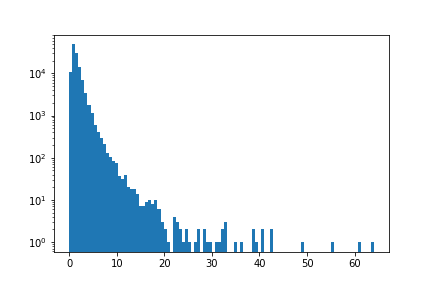
\includegraphics[width=12cm]{figures/TGL_hist.png}
    \caption{A trigliceridek hisztogramja logaritmikus skálán}
    \label{fig:cardio_tgl_hist}
\end{figure}

A trigliceridek változó értékeinek 100 vödörbe osztott hisztogramja a \ref{fig:cardio_tgl_hist}. ábrán található. Az \emph{y} tengely skálázása logaritmikus, így láthatók a kis értékek is. A 18-as értékig minden vödörbe legalább 10 adatpont esett, utána előfordulnak 0 és 1 adatot tartalmazó vödrök. Ilyen mennyiségű adatnál ezek kiugró értékeknek számítanak.

Ezért minden folytonos változó eredeti adatainak felső és alsó 5 percentilise eltávolítható az adatsorból, így a hibák nem kerülnek az algoritmus tanító adataiba. Az eredeti adatsorban így 80 462 adatpont marad, amely a tanításhoz így is túl sok, úgyhogy az adatoknak továbbra is 1\% adódik tanító adatnak.

Az ismert topológiai sorrend mellett a kísérlet elvégezhető az információelméleti alapon kiszámolt sorrenden is. Ekkor a sorrend \emph{B, C, D, E, A}-nak adódott.

\begin{table}[htp]\centering
\begin{tabular}{lccc}
    Változó       & Referencia tartomány & Ismert sorrend & Kezdeti sorrend \\ \hline
    Kor           & -                    & 39.18, 60.35   & 48.09           \\
    Koleszterin   & 0.9, 1.5             & 1.31, 1.58     & 1.15, 1.69      \\
    Trigliceridek & 0.5, 2.0             & 0.89, 1.60     & 0.69, 1.25      \\
    Vércukor      & 3.9, 5.8             & 4.75, 5.45     & 4.05, 5.25
    \end{tabular}
    \caption{A diszkretizációs határok a referencia tartományok szerint és az algoritmus ismert topológiai sorrenden történő futtatásával, kiugró értékek eltávolítása után.}
    \label{tab:cardio_kiugro_ertek}
\end{table}

\begin{figure}[htp]
    \centering
    \includegraphics[width=8cm]{figures/cardio/cardio_ismert.png}
    \caption{A tanult Bayes-háló az algoritmus ismert topológiai sorrenden történő futtatásával, kiugró értékek eltávolítása után.}
    \label{fig:cardio_kiugro_ertek}
\end{figure}

\begin{figure}[htp]
    \centering
    \includegraphics[width=8cm]{figures/cardio/cardio_kezdeti.png}
    \caption{A tanult Bayes-háló az algoritmus ismert topológiai sorrenden történő futtatásával, kiugró értékek eltávolítása után.}
    \label{fig:cardio_kiugro_ertek_kezdeti}
\end{figure}

Az így futtatott algoritmus a \ref{tab:cardio_kiugro_ertek}. táblázatban található referencia tartományokat állapítja meg. Az ismert sorrenddel futtatott algoritmus a \ref{fig:cardio_kiugro_ertek}. ábrán látható, a számolt kezdeti sorrenddel futtatott a \ref{fig:cardio_kiugro_ertek_kezdeti}. ábrán látható Bayes-hálót építi fel. Az ismert sorrend mellett is az eredetitől jelentősen eltérő háló az eredmény, tartalmaz olyan éleket, melyet az eredeti nem, valamint nem is lett összefüggő.

A referencia tartománytól a diszkretizációs határpontok így is eltérnek, de kapcsolat érzékelhető közöttük. Ez a módszer nem elégséges a referencia tartományok megtalálásához, de az elkészült Bayes-háló alkalmas lehet predikcióra.

\section{Koronavírus}
A predikciós képesség vizsgálatához másik adathalmazra volt szükség, mert ebben nem állt rendelkezésre előre jelzésre alkalmas változó. A 2020-as járványhelyzet miatt megjelent több adatsor is fertőzéssel kapcsolatos adatokkal.

Az Albert Einstein Kórház, São Paulo, Brazil által kiadott adatsort publikálta Avilla et al. \cite{avila2020hemogram}. A kórházban 5 644 páciensen végeztek qRT-PCR tesztet, mert COVID-19 fertőzésre utaló tüneteik voltak. Néhány személyről vérképet is készítettek, összesen 15 paraméter alapján. Teljes adat csak 510 páciensnél van, így a hiány jelentős. Az adatsor tartalmazza többek között a qRT-PCR teszt eredményét, a páciens azonosítóját egyirányúan titkosítva, a korcsoportját 5 éves csoportokban, valamint a vérkép eredményét az adott paraméter szerint normalizálva, hogy az anonimitást fenntartsák. A diszkrét változó a teszt eredménye, a többi folytonosnak tekinthető.

A Diplomaterv méréseibe a glükóz szintje nem volt használva, mert az volt a legtöbb helyen hiányzó adat. Így az 510 helyett 598 mintás adatsoron volt lehetőség futtatni az algoritmust. A topológiai sorrendet kizárólag az információelméleti megközelítésből származó feltételes entrópia algoritmus határozta meg, mert semmilyen előismeret nem volt a változók egymásra gyakorolt hatásával kapcsolatban. A maximális szülőszám 3-ban volt maximalizálva. A futtatás 646.781 másodpercet, vagyis 10 perc 47 másodpercet vett igénybe. Ennek legfőbb oka a nagyszámú változó és a sok tanult él a gráfban.

\begin{figure}[htp]
    \centering
    \includegraphics[width=15cm]{figures/covid/covid_result.png}
    \caption{A tanult Bayes-háló a koronavírus adatsoron}
    \label{fig:covid_result}
\end{figure}

A tanult Bayes-háló a \ref{fig:covid_result}. ábrán található. Feltűnő, hogy a vörösvértestekkel kapcsolatos paramétereket leválasztotta a teszteredményről, ez alapján függetlennek tekinthető lehetne. Másik érdekesség a kor változó is a vörösvértest fába került, azok méretével kapcsolatban. A teszt eredményének fája két ágra bomlik. Egyik a vérlemezkékkel kapcsolatos, másik az immunrendszerrel. Ez nem egy meglepő eredmény, de empirikusan alátámaszthatja az algoritmust.

\begin{figure}[htp]
    \centering
    \includegraphics[width=15cm]{figures/covid/covid_small.png}
    \caption{A tanult Bayes-háló a koronavírus adatsor részletén}
    \label{fig:covid_small_result}
\end{figure}

A megtanult hálóban a PCR teszt változó fája csak 8 változót tartalmaz. Ezekből is készíthető egy adatsor, melyen szintén futtatható az algoritmus. Az így tanult háló a \ref{fig:covid_small_result}. ábrán látható.It egy kicsit átrendeződött, mert a feltételes entrópiák a többi változó kimaradásával máshogy alakultak, így kissé más sorrendben tanulta a változókat, ám a legtöbb él ugyanaz maradt. Az előnye ennek, hogy így 86.843 másodperc alatt, azaz 1 perc 17 másodperc után lett eredmény. Ez 13.4\%-a az eredeti futási időnek, mely jelentős javulás a kevesebb változónak köszönhető.

\begin{table}[htp]\centering
\begin{tabular}{lcc}
    Metrika                         & Minden változó & Összefüggő változók \\ \hline
    Valódi pozitív                  & 492            & 486                 \\
    Hamis pozitív                   & 108            & 114                 \\
    Valódi pozitív arány            & 0.82           & 0.81                \\
    Hamis felfedezési arány         & 0.18           & 0.19                \\
    Pozitív prediktív érték         & 0.82           & 0.81                \\
    Pontosság                       & 0.82           & 0.81                \\
    Matthews korrelációs együttható & 0.64           & 0.62                \\
    F-pontszám                      & 0.82           & 0.81
    \end{tabular}
    \caption{A koronavírus adatsoron mért prediktív teljesítmények}
    \label{tab:covid_teljesitmeny}
\end{table}

A kiértékelést elvégezve az volt látható, hogy a Bayes-háló minden esetben negatív tesztet jósolt. Ennek oka, hogy a tanító adatsorban csak $\frac{1}{6}$ arányban szerepeltek pozitív tesztek. Ezeknek háromszoros súlyt adva a tanító adathalmazon hatszoros kereszt-validációt lehetett alkalmazni. Így megmérve az összes változóval, valamint csak a PCR teszttel összefüggő változókkal történő tanítást a \ref{tab:covid_teljesitmeny}. táblázat eredményei kaphatók. A kevesebb változó a prediktív teljesítményben nem okozott jelentős romlást, de kissé rosszabb eredményt ért el, mint az összes változón dolgozó.

Az adatsorhoz kapcsolódó tanulmányban \cite{avila2020hemogram} amikor a specificitást és érzékenységet is maximaziláltak, 76.7\%-os teljesítményt értek el. Ezek a metrikák pontosan megfelelnek rendre az \emph{1 - hamis felfedezési arány}, valamint a \emph{valódi pozitív arány} metrikáknak, melyek a Bayes-döntés alapú diszkretizációs algoritmussal 82\%-nak és 81\%-nak adódtak. Ez alapján az ezen algoritmussal készült Bayes-háló alkalmas predikcióra laboratóriumi paramétereken is.

%Értékelés
%Összefoglalás
%----------------------------------------------------------------------------
\chapter{Összefoglalás}
%----------------------------------------------------------------------------

A Diplomatervezés 1. tárgy során elkészítettem az ismertetett modul implementációját, valamint a Diplomamunkám néhány fejezetét elkészítettem. Ezek még bővítve lesznek, illetve a szintetikus és valós adatsoron történő kiértékelés még az elkészült Diplomamunka részét fogja képezni.

A Diplomamunka bemutat és megvalósít egy többváltozós diszkretizációs algoritmust. A bemutatás tartalmazza a megértéshez szükséges alapfogalmak magyarázatát, valamint a Bayes-elmélet azon részleteit, melyet a Bayes-hálók vagy az ismertetett algoritmus felhasznál.

Az ismertetett algoritmust egy modul részeként teszi könnyen felhasználhatóvá. A modul nyílt forráskódú, az elérés megtalálható a Függelékben. A használatát az \ref{chapter:modul}. fejezet írja le.

%Továbbfejlesztés
%Mutual information eredeti folytonos adatsoron

%\listoffigures\addcontentsline{toc}{chapter}{Ábrák jegyzéke}
%\listoftables\addcontentsline{toc}{chapter}{Táblázatok jegyzéke}

\printbibliography[title={Irodalomjegyzék}]
%\bibliography{mybib}
\addcontentsline{toc}{chapter}{Irodalomjegyzék}
%\bibliographystyle{plain}

%%----------------------------------------------------------------------------
\appendix \label{chapter:függelék}
%----------------------------------------------------------------------------
\chapter*{Függelék}\addcontentsline{toc}{chapter}{Függelék}
\setcounter{chapter}{6}  % a fofejezet-szamlalo az angol ABC 6. betuje (F) lesz
\setcounter{equation}{0} % a fofejezet-szamlalo az angol ABC 6. betuje (F) lesz
\numberwithin{equation}{section}
\numberwithin{figure}{section}
\numberwithin{lstlisting}{section}
%\numberwithin{tabular}{section}


%New colors defined below
\definecolor{codegreen}{rgb}{0,0.6,0}
\definecolor{codegray}{rgb}{0.5,0.5,0.5}
\definecolor{codepurple}{rgb}{0.58,0,0.82}
\definecolor{backcolour}{rgb}{0.95,0.95,0.92}

%Code listing style named "mystyle"
\lstdefinestyle{mystyle}{
  backgroundcolor=\color{backcolour},   commentstyle=\color{codegreen},
  keywordstyle=\color{magenta},
  numberstyle=\tiny\color{codegray},
  stringstyle=\color{codepurple},
  basicstyle=\ttfamily\footnotesize,
  breakatwhitespace=false,         
  breaklines=true,                 
  captionpos=b,                    
  keepspaces=true,                 
  numbers=left,                    
  numbersep=5pt,                  
  showspaces=false,                
  showstringspaces=false,
  showtabs=false,                  
  tabsize=2
}

\section{Kódbázis} \label{appendix:codebase}
Az implementáció során létrehozott nyílt forráskódú kód elérhető az alábbi linken: \\ \url{https://github.com/zihbot/tobbvaltozos-diszkretizacio}

\section{Egyszerű példa} \label{appendix:simpleexample}
\begin{lstlisting}
import bediscretizer
import sklearn.datasets

iris = sklearn.datasets.load_iris()
data = bediscretizer.util.concat_array(iris['data'], iris['target'])
d = bediscretizer.MultivariateDiscretizer(data, 'Iris')
d.fit()
d.draw_structure_to_file()
\end{lstlisting}

\label{page:last}
\end{document}
